% Options for packages loaded elsewhere
% Options for packages loaded elsewhere
\PassOptionsToPackage{unicode}{hyperref}
\PassOptionsToPackage{hyphens}{url}
%
\documentclass[
  english,
  russian,
  12pt,
  a4paper,
  DIV=11,
  numbers=noendperiod]{scrreprt}
\usepackage{xcolor}
\usepackage{amsmath,amssymb}
\setcounter{secnumdepth}{5}
\usepackage{iftex}
\ifPDFTeX
  \usepackage[T1]{fontenc}
  \usepackage[utf8]{inputenc}
  \usepackage{textcomp} % provide euro and other symbols
\else % if luatex or xetex
  \usepackage{unicode-math} % this also loads fontspec
  \defaultfontfeatures{Scale=MatchLowercase}
  \defaultfontfeatures[\rmfamily]{Ligatures=TeX,Scale=1}
\fi
\usepackage{lmodern}
\ifPDFTeX\else
  % xetex/luatex font selection
\fi
% Use upquote if available, for straight quotes in verbatim environments
\IfFileExists{upquote.sty}{\usepackage{upquote}}{}
\IfFileExists{microtype.sty}{% use microtype if available
  \usepackage[]{microtype}
  \UseMicrotypeSet[protrusion]{basicmath} % disable protrusion for tt fonts
}{}
\usepackage{setspace}
% Make \paragraph and \subparagraph free-standing
\makeatletter
\ifx\paragraph\undefined\else
  \let\oldparagraph\paragraph
  \renewcommand{\paragraph}{
    \@ifstar
      \xxxParagraphStar
      \xxxParagraphNoStar
  }
  \newcommand{\xxxParagraphStar}[1]{\oldparagraph*{#1}\mbox{}}
  \newcommand{\xxxParagraphNoStar}[1]{\oldparagraph{#1}\mbox{}}
\fi
\ifx\subparagraph\undefined\else
  \let\oldsubparagraph\subparagraph
  \renewcommand{\subparagraph}{
    \@ifstar
      \xxxSubParagraphStar
      \xxxSubParagraphNoStar
  }
  \newcommand{\xxxSubParagraphStar}[1]{\oldsubparagraph*{#1}\mbox{}}
  \newcommand{\xxxSubParagraphNoStar}[1]{\oldsubparagraph{#1}\mbox{}}
\fi
\makeatother


\usepackage{longtable,booktabs,array}
\usepackage{calc} % for calculating minipage widths
% Correct order of tables after \paragraph or \subparagraph
\usepackage{etoolbox}
\makeatletter
\patchcmd\longtable{\par}{\if@noskipsec\mbox{}\fi\par}{}{}
\makeatother
% Allow footnotes in longtable head/foot
\IfFileExists{footnotehyper.sty}{\usepackage{footnotehyper}}{\usepackage{footnote}}
\makesavenoteenv{longtable}
\usepackage{graphicx}
\makeatletter
\newsavebox\pandoc@box
\newcommand*\pandocbounded[1]{% scales image to fit in text height/width
  \sbox\pandoc@box{#1}%
  \Gscale@div\@tempa{\textheight}{\dimexpr\ht\pandoc@box+\dp\pandoc@box\relax}%
  \Gscale@div\@tempb{\linewidth}{\wd\pandoc@box}%
  \ifdim\@tempb\p@<\@tempa\p@\let\@tempa\@tempb\fi% select the smaller of both
  \ifdim\@tempa\p@<\p@\scalebox{\@tempa}{\usebox\pandoc@box}%
  \else\usebox{\pandoc@box}%
  \fi%
}
% Set default figure placement to htbp
\def\fps@figure{htbp}
\makeatother



\ifLuaTeX
\usepackage[bidi=basic,provide=*]{babel}
\else
\usepackage[bidi=default,provide=*]{babel}
\fi
% get rid of language-specific shorthands (see #6817):
\let\LanguageShortHands\languageshorthands
\def\languageshorthands#1{}


\setlength{\emergencystretch}{3em} % prevent overfull lines

\providecommand{\tightlist}{%
  \setlength{\itemsep}{0pt}\setlength{\parskip}{0pt}}



 
\usepackage[style=gost-numeric,backend=biber,langhook=extras,autolang=other*]{biblatex}
\addbibresource{bib/cite.bib}

\usepackage[]{csquotes}

\usepackage{indentfirst}
\usepackage{float}
\floatplacement{figure}{H}
\IfFileExists{plex-otf.sty}{
  %% Full TeXlive
  \usepackage[
    % math,
    RM={Scale=0.94},SS={Scale=0.94},SScon={Scale=0.94},TT={Scale=MatchLowercase,FakeStretch=0.9},
    DefaultFeatures={Ligatures=Common}
  ]{plex-otf}
  % \usepackage[Scale=MatchUppercase]{juliamono}
}{
  %% TinyTeX
  \usepackage{libertine}
}
\KOMAoption{captions}{tableheading}
\makeatletter
\@ifpackageloaded{caption}{}{\usepackage{caption}}
\AtBeginDocument{%
\ifdefined\contentsname
  \renewcommand*\contentsname{Содержание}
\else
  \newcommand\contentsname{Содержание}
\fi
\ifdefined\listfigurename
  \renewcommand*\listfigurename{Список иллюстраций}
\else
  \newcommand\listfigurename{Список иллюстраций}
\fi
\ifdefined\listtablename
  \renewcommand*\listtablename{Список таблиц}
\else
  \newcommand\listtablename{Список таблиц}
\fi
\ifdefined\figurename
  \renewcommand*\figurename{Рисунок}
\else
  \newcommand\figurename{Рисунок}
\fi
\ifdefined\tablename
  \renewcommand*\tablename{Таблица}
\else
  \newcommand\tablename{Таблица}
\fi
}
\@ifpackageloaded{float}{}{\usepackage{float}}
\floatstyle{ruled}
\@ifundefined{c@chapter}{\newfloat{codelisting}{h}{lop}}{\newfloat{codelisting}{h}{lop}[chapter]}
\floatname{codelisting}{Список}
\newcommand*\listoflistings{\listof{codelisting}{Листинги}}
\makeatother
\makeatletter
\makeatother
\makeatletter
\@ifpackageloaded{caption}{}{\usepackage{caption}}
\@ifpackageloaded{subcaption}{}{\usepackage{subcaption}}
\makeatother
\usepackage{bookmark}
\IfFileExists{xurl.sty}{\usepackage{xurl}}{} % add URL line breaks if available
\urlstyle{same}
\hypersetup{
  pdftitle={Отчёт по лабораторной работе №3},
  pdfauthor={Никита Сергеевич Паклин},
  pdflang={ru-RU},
  pdfkeywords={лабораторная работа, шаблон, Markdown, Pandoc},
  hidelinks,
  pdfcreator={LaTeX via pandoc}}


\title{Отчёт по лабораторной работе №3}
\usepackage{etoolbox}
\makeatletter
\providecommand{\subtitle}[1]{% add subtitle to \maketitle
  \apptocmd{\@title}{\par {\large #1 \par}}{}{}
}
\makeatother
\subtitle{Язык разметки Markdown}
\author{Никита Сергеевич Паклин}
\date{}
\begin{document}
\maketitle
\begin{abstract}
В данном отчёте представлены результаты выполнения лабораторной работы
по теме ``Язык разметки Markdown''

Описаны использованные методы, полученные экспериментальные данные и их
анализ.

Сделаны выводы о достижении поставленной цели.
\end{abstract}

\renewcommand*\contentsname{Содержание}
{
\setcounter{tocdepth}{1}
\tableofcontents
}
\listoffigures
\listoftables

\setstretch{1.5}
\chapter{Введение}\label{ux432ux432ux435ux434ux435ux43dux438ux435}

\section{Актуальность}\label{ux430ux43aux442ux443ux430ux43bux44cux43dux43eux441ux442ux44c}

Отчёты по всем последующим лабораторным работам курса оформляются в
Markdown. Markdown - простой текстовый формат: его удобно хранить в git,
отслеживать изменения и из одного файла получать отчёт сразу в
нескольких форматах (PDF, DOCX).

\section{Цель
работы}\label{ux446ux435ux43bux44c-ux440ux430ux431ux43eux442ux44b}

Освоение процедуры оформления отчетов с помощью легковесного языка
разметки Markdown.

\section{Задачи}\label{ux437ux430ux434ux430ux447ux438}

\begin{enumerate}
\def\labelenumi{\arabic{enumi}.}
\tightlist
\item
  Скомпилировать шаблон отчёта с помощью Makefile и проверить полученные
  файлы.
\item
  Удалить полученные файлы с помощью Makefile.
\item
  Изучить структуру файла отчёта.
\item
  Заполнить отчёт и скомпилировать его в форматы PDF и DOCX.
\item
  Загрузить файлы в репозиторий на GitVerse.
\item
  Оформить в Markdown отчёт по лабораторной работе № 2.
\end{enumerate}

\section{Объект и предмет
исследования}\label{ux43eux431ux44aux435ux43aux442-ux438-ux43fux440ux435ux434ux43cux435ux442-ux438ux441ux441ux43bux435ux434ux43eux432ux430ux43dux438ux44f}

Объект - шаблон отчёта по лабораторной работе. Предмет - синтаксис
Markdown и процесс преобразования Markdown-файла в форматы PDF и DOCX.

\section{Методы
исследования}\label{ux43cux435ux442ux43eux434ux44b-ux438ux441ux441ux43bux435ux434ux43eux432ux430ux43dux438ux44f}

Практическое выполнение команд в терминале Linux, редактирование файла
отчёта в текстовом редакторе, проверка результата компиляции.

\chapter{Теоретическая
часть}\label{ux442ux435ux43eux440ux435ux442ux438ux447ux435ux441ux43aux430ux44f-ux447ux430ux441ux442ux44c}

Markdown - легковесный язык разметки: оформление задаётся простыми
символами прямо в тексте. Основные элементы приведены в табл.
\textbf{?@tbl-md}. Элемент Запись в Markdown Заголовок 1 уровня \#
Heading Полужирный \textbf{text} Курсив \emph{text} Нумерованный список
1. item Маркированный список - item Ссылка \href{url}{text} Изображение
\pandocbounded{\includegraphics[keepaspectratio]{path.pdf}} : Основные
элементы разметки Markdown \{\#tbl-md\} Формулы записываются в
синтаксисе LaTeX: внутри строки - между \$, например
\(\sin^2(x) + \cos^2(x) = 1\); отдельной строкой - между \$\$ с меткой
для ссылки:

\sin\^{}2(x) + \cos\^{}2(x) = 1

\{\#eq-trig\} На формулу (\textbf{?@eq-trig}) можно сослаться по её
метке \textbf{?@eq-trig}, на рисунок - по метке \textcite{fig}-\ldots,
на таблицу - по метке \textcite{tbl}-\ldots. Материалы и методы Работа
выполнена в ОС Fedora. Использованное программное обеспечение: Quarto
1.7.34 - компиляция Markdown в PDF и DOCX (рис. \textbf{?@fig-quarto});
TinyTeX - дистрибутив LaTeX для сборки PDF; make - запуск команд из
Makefile; git - работа с репозиторием; gedit - редактирование отчёта.

\chapter{Выполнение лабораторной
работы}\label{ux432ux44bux43fux43eux43bux43dux435ux43dux438ux435-ux43bux430ux431ux43eux440ux430ux442ux43eux440ux43dux43eux439-ux440ux430ux431ux43eux442ux44b}

Выполнен переход в каталог курса командой cd, локальный репозиторий
обновлён командой git pull (рис. \textbf{?@fig-pull}). Ответ «Уже
актуально» означает, что новых изменений на сервере нет.
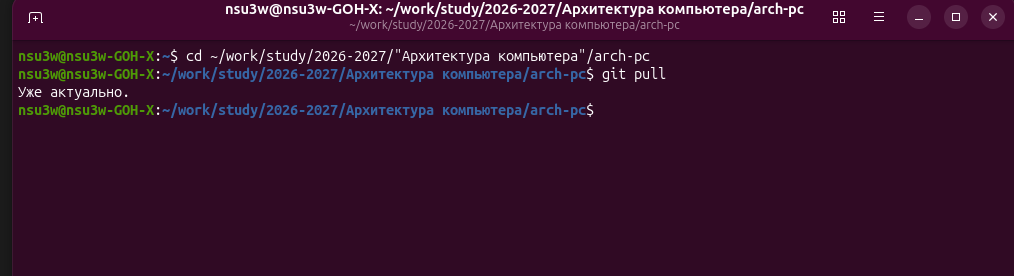
\includegraphics[width=0.9\linewidth,height=\textheight,keepaspectratio]{image/git-pull.png}

Выполнен переход в каталог labs/lab03/report. Команда ls показала его
содержимое: Makefile, файл настроек \_quarto.yml, файл отчёта
arch-pc-lab03-report.qmd и каталог image для изображений (рис.
\textbf{?@fig-ls}).
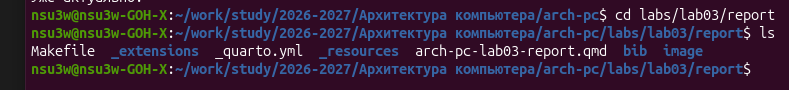
\includegraphics[width=0.9\linewidth,height=\textheight,keepaspectratio]{image/ls-report.png}

Команда make выполнила цель all из Makefile, которая запускает quarto
render. В каталоге \_output сформированы файлы отчёта в форматах PDF и
DOCX (рис. \textbf{?@fig-make}).
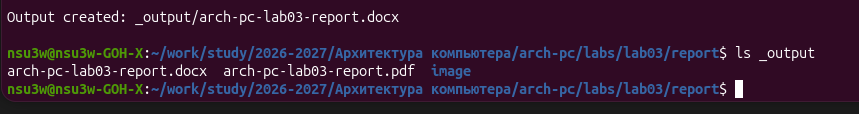
\includegraphics[width=0.9\linewidth,height=\textheight,keepaspectratio]{image/make.png}
При проверке PDF обнаружено, что блок-схема из шаблона не отрисовалась
(рис. \textbf{?@fig-mermaid}): она записана в синтаксисе mermaid версии
11.3, а в Quarto 1.7.34 встроена версия 11.2.0. Поэтому схема была
удалена из отчёта.
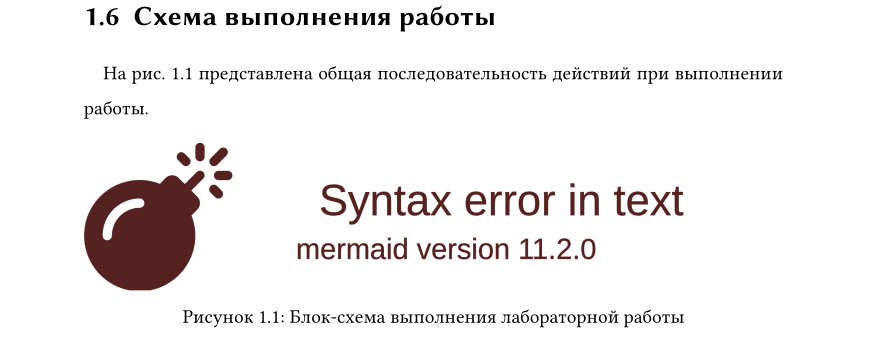
\includegraphics[width=0.8\linewidth,height=\textheight,keepaspectratio]{image/pdf-mermaid-error.png}

Команда make clean выполнила rm -rf \_output и удалила каталог с
готовыми файлами (рис. \textbf{?@fig-clean}). Содержимое каталога
совпало с исходным.
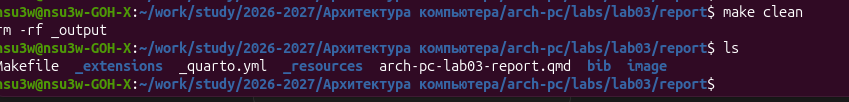
\includegraphics[width=0.9\linewidth,height=\textheight,keepaspectratio]{image/make-clean.png}

Файл отчёта открыт в текстовом редакторе (рис. \textbf{?@fig-editor}).
Он состоит из YAML-шапки между строками - (автор, название, аннотация) и
текста отчёта, размеченного Markdown. Скриншоты размещаются в каталоге
image.
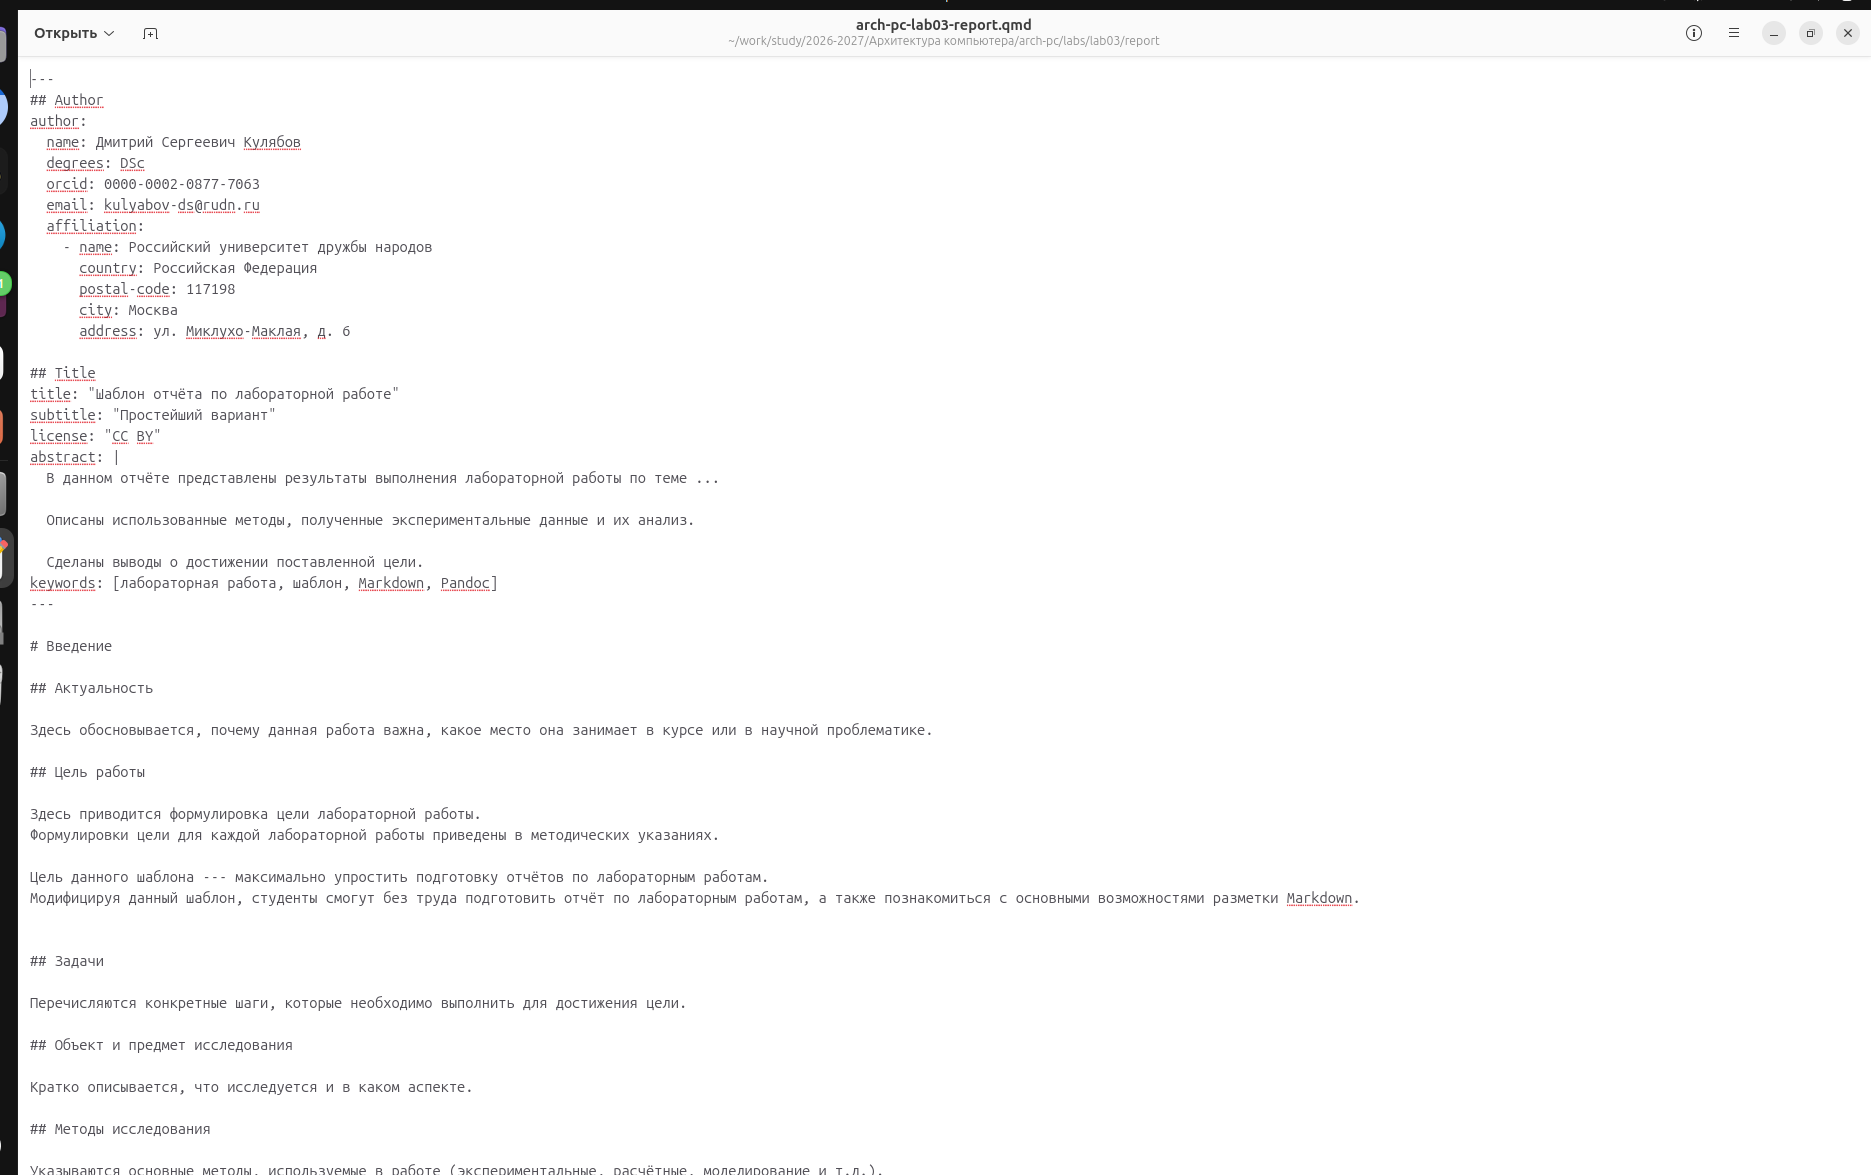
\includegraphics[width=0.9\linewidth,height=\textheight,keepaspectratio]{image/qmd-editor.png}

В шапке указаны автор, название и аннотация. Примеры из шаблона удалены,
разделы заполнены описанием выполненной работы. Отчёт скомпилирован
командой make (рис. \textbf{?@fig-report}).

\includegraphics[width=0.6\linewidth,height=\textheight,keepaspectratio]{image/report-pdf.png}

Изменения добавлены в индекс командой git add ., сохранены коммитом git
commit -am \enquote*{feat(main): add files lab-3} и отправлены на GitHub
командой git push (рис. \textbf{?@fig-push}). Строка master
-\textgreater{} master подтверждает обновление ветки на сервере.
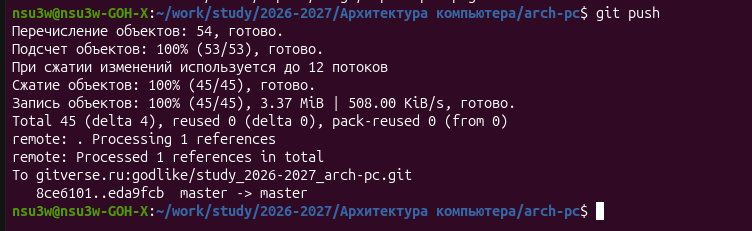
\includegraphics[width=0.9\linewidth,height=\textheight,keepaspectratio]{image/git-push.png}

\section{Самостоятельная
работа}\label{ux441ux430ux43cux43eux441ux442ux43eux44fux442ux435ux43bux44cux43dux430ux44f-ux440ux430ux431ux43eux442ux430}

В каталоге labs/lab02/report отчёт по лабораторной работе № 2 оформлен в
формате Markdown и скомпилирован в форматы PDF и DOCX. Репозиторий с
отчётами: https://github.com/AlmerDiamond/study\_2026-2027\_arh-pc

\chapter{Результаты}\label{ux440ux435ux437ux443ux43bux44cux442ux430ux442ux44b}

\begin{itemize}
\tightlist
\item
  Шаблон отчёта скомпилирован и очищен с помощью Makefile.
\item
  Подготовлен отчёт по лабораторной работе № 3 в форматах Markdown, PDF
  и DOCX.
\item
  Отчёт по лабораторной работе № 2 переоформлен в Markdown.
\item
  Файлы загружены в репозиторий на GitVerse.
\end{itemize}

\chapter{Обсуждение
результатов}\label{ux43eux431ux441ux443ux436ux434ux435ux43dux438ux435-ux440ux435ux437ux443ux43bux44cux442ux430ux442ux43eux432}

Компиляция прошла успешно, однако проверка PDF показала, что успешное
завершение make не гарантирует корректность документа: блок-схема
шаблона не отрисовалась из-за несовпадения версий mermaid. Поэтому
полученные файлы необходимо просматривать после каждой сборки.

\chapter{Заключение}\label{ux437ux430ux43aux43bux44eux447ux435ux43dux438ux435}

\begin{itemize}
\tightlist
\item
  Цель работы достигнута: освоена процедура оформления отчётов с помощью
  Markdown.
\item
  Изучены синтаксис Markdown, оформление изображений, таблиц и формул со
  ссылками на них.
\item
  Освоена компиляция отчёта в PDF и DOCX с помощью Quarto и Makefile.
\end{itemize}


\printbibliography



\end{document}
